\documentclass{standalone}

% graphics
\usepackage{tikz}
\usepackage{pgfplots}
\usepackage{siunitx}

\begin{document}

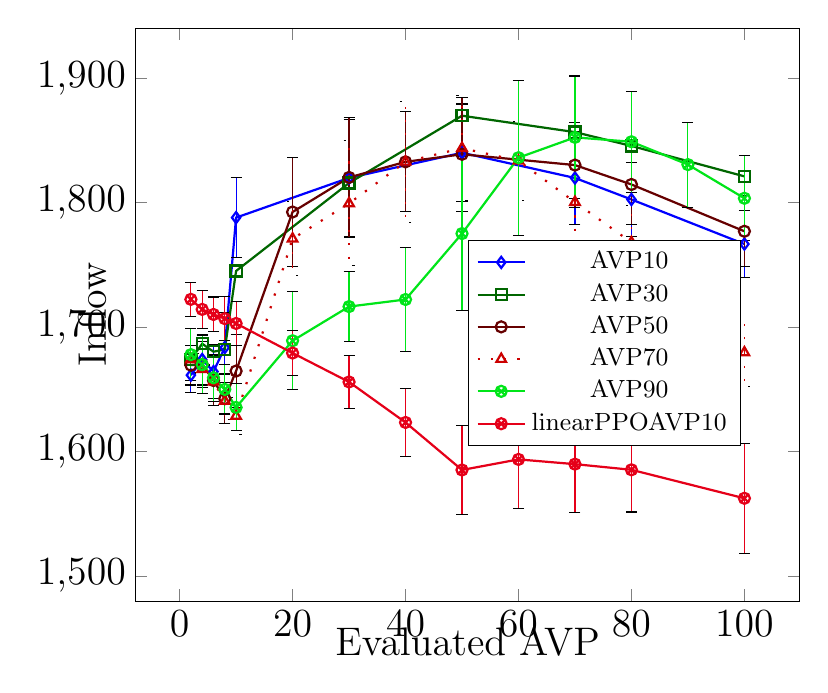
\begin{tikzpicture}[scale=1]
  \pgfplotsset{
      scale only axis,
      every x tick label/.append style={font=\Large},
      every y tick label/.append style={font=\Large},
	legend style={at={(0.5,0.63)},anchor=north west}
  }

\begin{axis}[
    legend style={font=\small},
	ylabel={\Large Inflow},
	x label style={at={(axis description cs:0.5,-0.03)},anchor=north},
	y label style={at={(axis description cs:-0.030,0.5)}, anchor=south},
	xlabel={\Large Evaluated AVP},
]
% trained on avp=10 
% dashdotdotted,
\addplot[mark=diamond, thick, mark options={solid, fill=blue!40, mark size=2 pt}, draw=blue, error bars/.cd, y dir=both, y explicit] table [x=a, y=b, y error=c] {
a	b   	c
2 1661.33 14.01
4 1673.89 20.45
6 1664.21 21.66
8 1683.54 28.42
10 1787.94 32.12
30 1819.87 46.89
50 1840.07 39.22
70 1819.80 37.26
80 1802.52 30.07
100 1766.70 27.21
};
\label{AVP10}

% trained on avp=30
% error bars/.cd, y dir=both, y explicit,
\addplot[mark=square, thick, mark options={solid, fill=green!60, mark size=2 pt}, draw=black!60!green] table [x=a, y=b] {
a	b   	c
2 1674.14 16.52
4 1686.56 22.00
6 1680.16 23.40
8 1682.03 25.08
10 1745.06 33.26
30 1815.77 51.27
50 1869.84 47.53
70 1856.66 34.37
80 1845.54 34.82
100 1821.10 31.43
};
\label{AVP30}  

%densely dashed, 
\addplot[mark=o, thick, mark options={solid, fill=black!60!red, mark size=2pt}, draw=black!60!red, error bars/.cd, y dir=both, y explicit] table [x=a, y=b, y error=c] {
a	b   	c
2 1669.36 15.98
4 1669.86 18.20
6 1657.01 20.07
8 1642.43 19.79
10 1664.64 29.23
20 1792.44 44.02
30 1820.23 48.34
40 1832.76 40.13
50 1838.84 45.92
70 1830.17 33.98
80 1814.58 32.04
100 1776.96 28.64
};
\label{AVP50}

%densely dashed, 
\addplot[mark=triangle, thick, loosely dotted, mark options={solid, fill=red!60, mark size=2pt}, draw=black!20!red, error bars/.cd, y dir=both, y explicit] table [x=a, y=b, y error=c] {
a	b   	c
2 1674.00 10.90
4 1666.12 12.79
6 1656.00 13.50
8 1640.63 14.85
10 1628.53 14.67
20 1770.95 29.81
30 1799.35 50.23
40 1832.76 48.80
50 1843.74 42.08
60 1833.62 31.62
70 1800.36 32.69
80 1768.03 29.51
100 1679.47 27.41
};
\label{AVP70}

%densely dashed, 
\addplot[mark=otimes, thick, mark options={solid, fill=red!60, mark size=2pt},
draw=blue!10!green, error bars/.cd, y dir=both, y explicit] table [x=a, y=b, y error=c] {
a	b   	c
2 1677.82 21.13
4 1669.82 23.12
6 1659.24 18.82
8 1649.88 19.75
10 1635.41 18.87
20 1688.98 39.40
30 1716.44 28.40
40 1722.13 41.84
50 1775.12 61.71
60 1836.11 62.33
70 1852.42 49.37
80 1848.92 40.73
90 1830.56 34.15
100 1803.49 34.20
};
\label{AVP90}

%\addplot[mark=none, black, samples=2] {2184.91};\label{Baseline}

%densely dashed, 
\addplot[mark=otimes, thick, mark options={solid, fill=blue!60, mark size=2pt},
draw=blue!10!red, error bars/.cd, y dir=both, y explicit] table [x=a, y=b, y error=c] {
a	b   	c
2 1722.24 13.45
4 1714.18 15.35
6 1710.11 14.00
8 1706.76 17.78
10 1702.87 17.82
20 1679.11 17.95
30 1655.86 21.62
40 1623.31 27.50
50 1585.12 35.44
60 1593.61 39.77
70 1589.80 38.61
80 1585.26 33.93
100 1562.36 44.24
};
\label{linearPPO}


\addlegendimage{/pgfplots/refstyle=AVP10}
\addlegendentry{AVP10}

\addlegendimage{/pgfplots/refstyle=AVP30}
\addlegendentry{AVP30}

\addlegendimage{/pgfplots/refstyle=AVP50}
\addlegendentry{AVP50}

\addlegendimage{/pgfplots/refstyle=AVP70}
\addlegendentry{AVP70}

\addlegendimage{/pgfplots/refstyle=AVP90}
\addlegendentry{AVP90}

\addlegendimage{/pgfplots/refstyle=linearPPO}
\addlegendentry{linearPPOAVP10}


%\addlegendimage{/pgfplots/refstyle=Baseline}
%\addlegendentry{Human Baseline}




\end{axis}
\end{tikzpicture}

\end{document}

